%In the next application, a benchmark sends a constant rate of http requests to a single threaded webserver deployed using the http module running inside a nodejs process. In contrast to the simplified round trip behavior of netpipe, this webserver incurs a heavier processing burden.  Across 
% Even in this regime, tuning hardware knobs matters in both Linux and the library OS
%\begin{table}[]
%\begin{tabular}{| c | c | c | c | c | c |}
%\hline
%           & \multicolumn{4}{c |}{Latency ($\micro$s)} &   \\ \hline
%           & 50\% & 75\% & 90\% & 99\% &  Requests\\ \hline
%\begin{tabular}{@{}c@{}}Linux \\ Default\end{tabular}    & 81   & 82   & 85   & 91   & 365758         \\ \hline
%\begin{tabular}{@{}c@{}}Linux \\ Tuned\end{tabular}    & 74   & 76   & 79   & 85   & 394704         \\ \hline
%\begin{tabular}{@{}c@{}}Library OS\\ Tuned\end{tabular} & 59   & 60   & 61   & 68   & 491765         \\ \hline
%\end{tabular}
%\caption{NodeJS Performance Data}
%\label{tab:nodejs}
%\end{table}
%% across the latencies, variance is mostly similar, 99% tail latency is this, and translates to this throughput

%Table~\ref{tab:nodejs} illustrates the base performance of running a webserver in nodejs. Linux tuned is able to achieve 8\% higher requests than default just by disabling its default DVFS and itr-delay policy and selecting a set of static values that maximizes its performance, while the library OS improves performance by 35\%. With
% for computational work you do have to do, if 
\begin{figure}[t]
	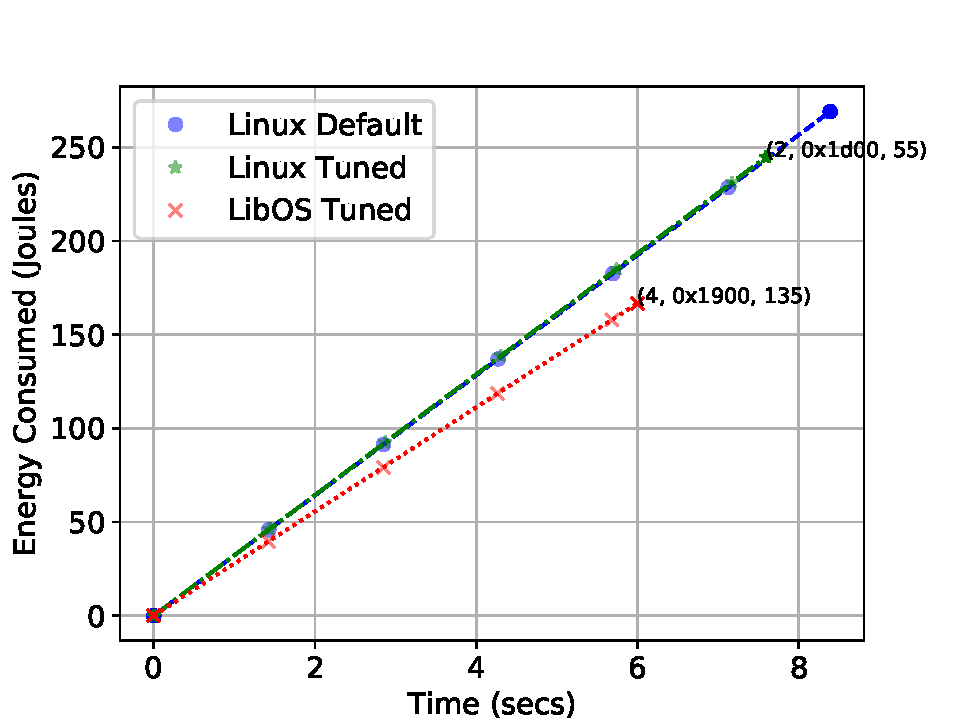
\includegraphics[width=\columnwidth]{osdi_figures/nodejs_edp.pdf}
	\caption{NodeJS EPP plot across three systems}
	\label{fig:nodejs_epp}
\end{figure}
\begin{figure}[t]
	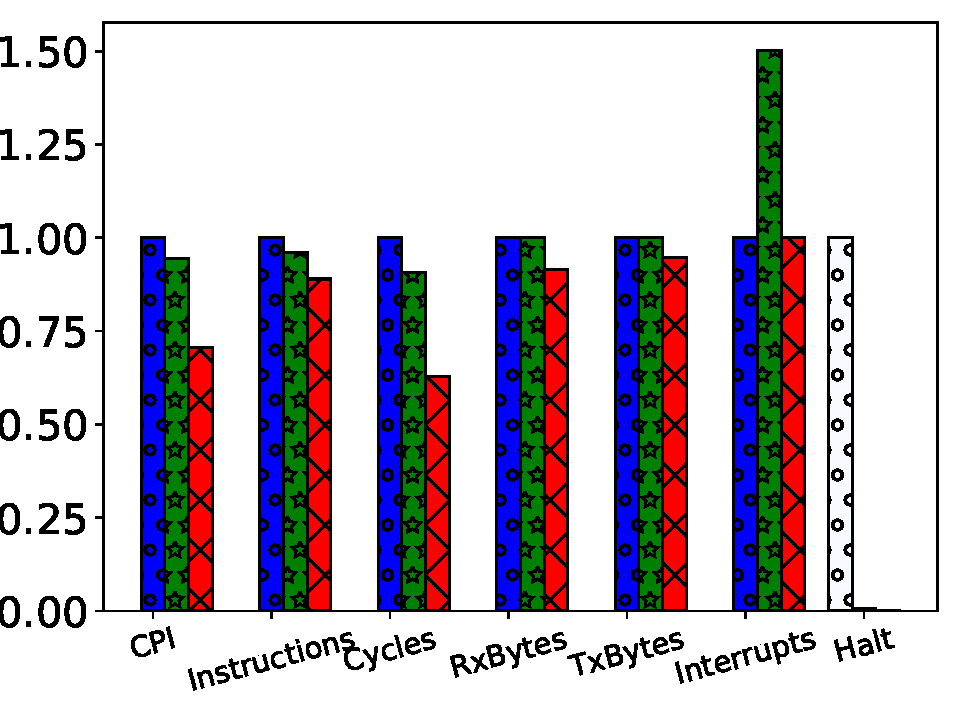
\includegraphics[width=\columnwidth]{osdi_figures/nodejs_barplot.pdf}
	\caption{Collected datapoints of NodeJS across three systems normalized to Linux Default}
	\label{fig:nodejs_bar}
\end{figure}
\begin{figure}[t]
	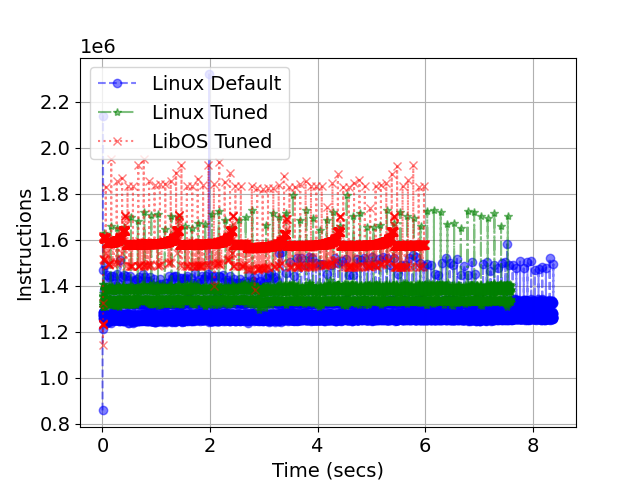
\includegraphics[width=\columnwidth]{osdi_figures/nodejs_instructions_timeline.png}
	\caption{NodeJS: Per interrupt instruction count.}
	\label{fig:nodejs_instruction}
\end{figure}

\subsubsection{General Observations}
In contrast to NetPIPE, with the move to a processing heavier workload, we found the top minimum EPP points all used ITR delay values of 2 and 4 \micro s for both tuned Linux and the libOS. The efficiency of the libOS over Linux is more dramatic here as the minimum EPP for Linux tuned all required setting DVFS at the higher frequencies (0x1b00-0x1d00), whereas the libOS is still able to lower its processor frequency (0x1900-0x1b00) to conserve additional energy. For the minimum EPP of Linux tuned, DVFS was set at the highest setting along with RAPL while ITR delay was set at lowest value of 2 \micro s. Given these settings, tuning Linux was able to lower its EPP over Linux default by 16\%, the libOS was able to lower its EPP of Linux default by 55\%. In both tuned settings, it was a combination of both savings in energy and time that contributed to the overall EPP.

\subsubsection{Slow to stay busy}
Past researchers have observed there is a tension between using controls like DVFS and RAPL to throttle energy consumption at some budget versus the savings that can be gained by finishing work quick and halting into idle states between the requests for work \cite{} -this latter strategy is often referred to as "race-to-halt" (r2h). In this work, we present a new effect of using processor frequency tuning as a way to "slow-to-stay-busy" s2sb, we found s2sb is only uniquely applicable in the run-to-completion model in the libOS. This was discovered by noticing dramatic decreases in number of interrupts (up to 100X) in NodeJS as DVFS was set to a very low processor frequency. Moreover, we found the bytes transmitted and received did not differ as dramatically from Linux. Upon closer examination of the libOS' receive path, we found the effect of a low DVFS setting is such that on the firing of a receive interrupt, it then has to rewind all the back to the original receive handling code after transmitting a reply, the lowered processor frequency causes this entire process to be slowed down. Moreover, the libOS' receive code is written such that it will poll the NIC for additional packets up to a certain limit, this limit is based upon values used in~\cite{}. Therefore once the code has slowly returned to the receive interrupt handler, it is possible that new packets have already arrived from the client and the libOS begins the process anew. The effect of low DVFS on a run-to-completion based OS is inducing this form of polling, which is based outside of its original intended design.

\subsubsection{NodeJS Analysis}
Similar to NetPIPE, the NodeJS experiment does not induce concurrent load as it is a single stream of serial transactions.  In this case, the client submits requests to a web server written in JavaScript.  This experiment lets us analyze hardware tuning in a application that contains a greater path length in processing every request, in addition the actual data communicated per client-server exchange is small (less than a MTU).  

%In order to present nodejs in a meaningful way with respect to EPP, we selected one sample run of each system hardware configuration with minimzed EDP and scaled the log data to show a fixed workload of up to 100K requests versus using the entire 30 second run.

Given that our load is slightly more realistic, it is natural to ask how the quality of service is impacted by tuning for minimum EPP by considering the measured 99\% tail latency.   For Linux default it is 92 \micro s, Linux tuned at 86 \micro s, and libOS at 66 \micro s.  Thus, static tuning of the hardware parameters yields lower request latency values than the default Linux behaviour of dynamically adjusting the values.

%These latency results also directly %translate to throughput gains given the single connection nature of this benchmark, with an 8\% improvement and 35\% improvement over Linux default by Linux tuned and the the library OS respectively.

% fixed tuning what kind of benefit over base Linux,
% what influence does having shorter code paths on tuning, 
% what does getting to sleep/idleness difference, 
% are you exploiting to sleep, synergistic with instruction efficiency,

Figure~\ref{fig:nodejs_epp} shows that tuning Linux is able to achieve a 8.5\% decrease in both time and energy to service 100K requests, however, the rate with which tuned Linux consumed energy did not change relative to default. Figure~\ref{fig:nodejs_bar} show some surprising differences in the two Linux configurations: 1) Linux default measured 200K total interrupts (100K for each incoming request and 100K for each outgoing transmit complete), however Linux tuned required 300K total interrupts instead (50\% increase) ; 2) Linux default called the \texttt{halt} instruction over 60K times while Linux tuned called the \texttt{halt} instructions 600 times, in both cases 99.99\% of \texttt{halt} states were \texttt{C1}; 3) Linux tuned used fewer instructions and cycles than Linux default and has a 5\% improvement in CPI. Linux's idling function~\cite{linux_idle} states that a \texttt{C1} state has a residency value of 2 \micro s, which is exactly the ITR delay value set for Linux tuned, moreover, figure~\ref{fig:nodejs_timediff} plots the time difference between interrupts and it is possible to see three major bands of interrupt delays, one for receive packet process, transmit completion, and another for the spurious interrupt that the hardware generates at low ITR delay values. These interrupts must be directly interferring with Linux's idling scheduler and is preventing it from going into any sleep states at all, and yet tuning Linux is still able to finish the workload quicker with lower energy usage. This must mean tuned Linux is being placed in a sort of polling mode due to impact of tuning ITR delay, this can be seen in the per-interrupt instruction differences as shown in figure~\ref{fig:nodejs_instruction}, one can see that after every interrupt, tuned Linux manages to be more instruction efficient in terms handling the request. This example also shows cases where it is actually more energy efficient to just poll and finish the work as soon as possible versus taking advantage of any idling. This enforced polling mode might also be the cause of the 5\% improvement in CPI of tuned Linux over its default counterpart.


Figure~\ref{fig:nodejs_epp} also shows tuned libOS is able to achieve a 37\% decrease in energy and 27\% decrease in time to service 100K requests and at a lower rate of energy consumption than Linux default. While the libOS also uses a low ITR delay value of 4 \micro s, figure~\ref{fig:nodejs_bar} shows that its number of interrupts is still similar to Linux default even though its number of \texttt{halt} counts is similar to Linux tuned, meaning the libOS did not have any opportunities to idle. There are two factors contributing to this: 1) the libOS uses shorter packet processing path lengths even though the libOS is running the V8 JavaScript engine executing a HTTP webserver - this is shown in its 30\% CPI improvement over Linux, and 2) the libOS uses a lower DVFS value than Linux and as shown from the findings section, the \textbf{S2SB} effect is in play here by artifically inducing a polling mode inside the libOS.


%We observe that as expected the number of instructions that each system has to execute is dominated by a fixed overhead due likely to the V8 javascript engine executing the javascript webserver.  However, we do see a small drop in instructions executed by the library OS. Given that it does not suffer the increase in interrupt processing we can conclude that the drop is likely from its shorter path lengths.

%Thus it seems we had reduction in work that yields a proportional reduction in total energy consumed.  Looking at figure~\ref{fig:nodejs_bar} we in-fact do see a small drop in the instructions executed and a proportional drop in energy and cycles. 

%While at first it may seem odd that there is a significant increase in interrupts one needs to account for the rate of interrupts that each system is realizing.  Analyzing the log files reveals that the rate of interrupts that Linux Tuned realizes is 40\%  faster than Linux Default.  This faster rate results in more interrupts given that the total time taken by Linux Tuned is only 10\% less than for Linux Default.  On the other hand the library OS rate of interrupts is 27\% faster but it also completes the work in 30\% less time.   These ratios result in the library OS using about the same number of interrupts to do the work as the default while the Linux Tuned spends more interrupts to do the work. 


%Tuning the library OS we find more significant advantages with respect to both reducing energy and time; 37\% and 27\% respectively compared to Linux default.  To understand this consider Figures~\ref{fig:nodejs_joules} and ~\ref{fig:nodejs_non_idle} in context of the Instruction, Energy and Ref. Cycles bars of figure~\ref{fig:nodejs_bar}.  We observe that as expected the number of instructions that each system has to execute is dominated by a fixed overhead due likely to the V8 javascript engine executing the javascript webserver.  However, we do see a small drop in instructions executed by the library OS.  Given that it does not suffer the increase in interrupt processing we can conclude that the drop is likely from its shorter path lengths.

%The drop in Energy and Ref Cycles when put in context of the joules consumed and non-idle time suggest that again while the cpu utilization is considerable compared to netpipe the library OS still manages to extract more opportunities to idle. To gain the ability to more rapidly complete the work per interrupt, given the mean utilization of 85\% between interrupts, versus the close to 100\% utilization for both Linux and Linux tuned,  is converted into more opportunities to reach an efficient idle behaviour between interrupt processing.    

%While there are many more details to the data we have gathered in interesting aspects to discuss, given space constraints we limiting our analysis.  

%27 time reduction 
% 37 %
%Partly it is due to the computationally heavier nature of this application, which for tuned Linux resulted in using over 40\% more interrupts than default as shown in figure~\ref{fig:nodejs_bar}. Intuitively, one would consider an increase in interrupts to correspond with more instructions due to more interrupt handling code and potentially more energy use. However, figure~\ref{fig:nodejs_bar} also shows neither to be the case in tuned Linux versus default, moreover, figure~\ref{fig:nodejs_non_idle} also shows tuned Linux did not get opportunities to idle as well. While tuned Linux was busier, it did not necessarily translate to more redundant work such as packet re-transmissions as figure~\ref{fig:nodejs_bar} shows a slight decrease in total transmitted bytes compared to default. Lastly, this Linux results implies that an for application like nodejs, minimizing overall time spent, or for performance, is the sole metric with which to save energy.

%In both Linux and the library OS tuned, an interrupt-delay of 4 us was selected, which suggests the importance of relying on a small static interrupt-delay value. Figure~\ref{fig:nodejs_edp} shows that tuning the library OS results in a 40\% decrease in time spent while also consuming energy at a reduced rate. While the library OS only used slightly lower instructions as shown in figure~\ref{fig:nodejs_bar}, the spread of energy use per interrupt is more telling of its efficiencies as shown in figure~\ref{fig:nodejs_joules}. This figure indicates that the library OS is consistently using less joules than Linux across the two main bands where work is actively being done. Further, these instruction efficiencies translate into potential processing slack, thereby allowing the library OS idle more as shown in figure~\ref{fig:nodejs_non_idle}.

%\begin{figure}
%	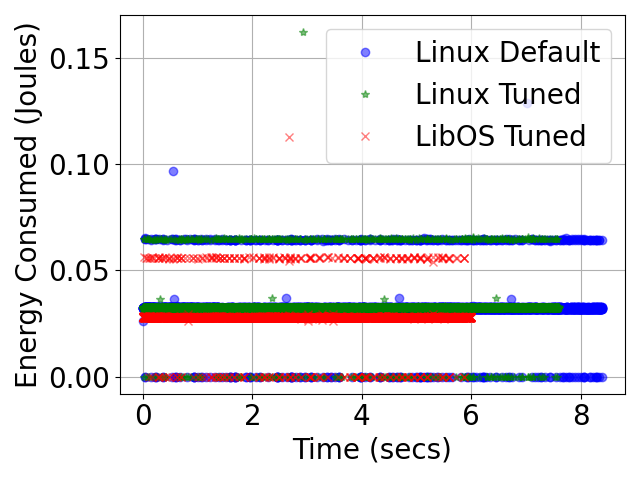
\includegraphics[width=\columnwidth]{osdi_figures/nodejs_joule_timeline.pdf}
%	\caption{NodeJS: Per interrupt measure of Joule}
%	\label{fig:nodejs_joules}
%\end{figure}

%results in aless dramatic difference in overall energy usage. 

%lower instruction -> lower energy, greater efficiency in instruction and potential to sleep more

%ref cycle 
